\myheader{Guía 1: Señales en el tiempo}

\begin{ejercicio}
    Sea $d_T(t)=t-T$ la función desplazamiento a derecha ($T>0$) y $e_a(t)=\frac{t}{a}$ la función expansión ($a > 1$). Para la señal $x(t)$
    
    \begin{align*}
        \inciso \parbox{.3\textwidth}{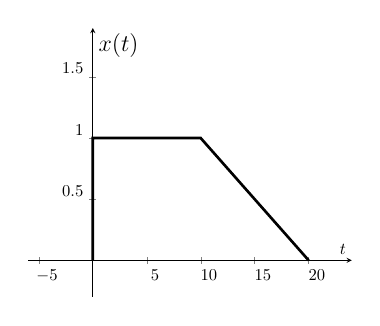
\begin{tikzpicture}[scale=0.6,transform shape]
    \begin{axis}[
    	axis y line=center,
    	axis x line=middle,
    	xlabel=$t$,ylabel={\Large $x(t)$},
    	xmin=-6,xmax=24,
    	ymin=-0.3,ymax=1.9,
    	xticklabel style = {xshift=5},
    	yticklabel style = {yshift=5},
    	]
    	\addplot[
    	black,
    	ultra thick
    	] coordinates {
    	    (0,0) (0,1) (10,1) (20,0)
    	};
    \end{axis}
\end{tikzpicture}
} & \hfill & \inciso \parbox{.3\textwidth}{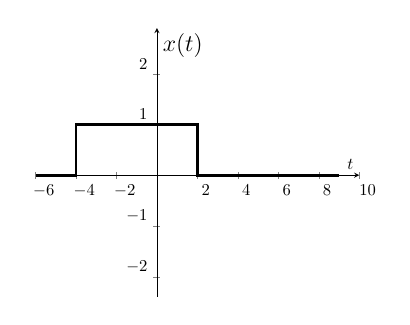
\begin{tikzpicture}[scale=0.6,transform shape]
    \begin{axis}[
    	axis y line=center,
    	axis x line=middle,
    	xlabel=$t$,ylabel={\Large $x(t)$},
    	xmin=-6,xmax=10,
    	ymin=-2.4,ymax=2.9,
    	xticklabel style = {xshift=5},
    	yticklabel style = {yshift=6},
    	]
    	\addplot[
    	black,
    	ultra thick
    	] coordinates {
    	    (-6,0) (-4,0) (-4,1) (0,1) (2,1) (2,0) (9,0)
    	};
		\diracdelta{4}{2};
		\diracdelta{7}{-2};
    \end{axis}
\end{tikzpicture}
}    
    \end{align*}
   
    graficar:
    \begin{align*}
        \subinciso x(d_1(e_2(t))) & \hfill & \subinciso x(e_2(d_1(t))) & \hfill & \subinciso x\left(\frac{3}{2}t + 1\right) \\  \subinciso x\left(-2t -1\right) & \hfill & \subinciso x\left(\frac{t}{2} - \frac{1}{2} \right) & & \hfill
    \end{align*}
    
\end{ejercicio}

\begin{ejercicio}
    Graficar esquemáticamente las siguientes señales de tiempo continuo y determinar si son periódicas o no.

    \inciso $x(t) = \cos(\frac{2\pi}{8} t)$

    \inciso $x(t) = \sin(\pi t) + \sin(\frac{2\pi}{3} t)$

    \inciso $x(t) = u(t-3) - u(t-5)$

    \inciso $x(t) = \int_{-\infty}^{\infty} \delta(t-4) - \delta(t-6)$

    \inciso Sinc normalizada: \begin{equation*}
        x(t) = \mathrm{sinc}(t) = 
        \begin{cases}
            \frac{\sin(\pi t)}{\pi t}    & \mbox{si } t \neq 0 \\[0.5em]
            1 & \mbox{si } t = 0    
        \end{cases}
    \end{equation*}

    \inciso Sinc periódica normalizada con $N=4$: \begin{equation*}
        x(t) = \mathrm{psinc}(t) = \begin{cases}
             \frac{\sin(N \pi t)}{N \sin(\pi t)} & \mbox{si } t \notin \Z \\[0.5em]
            (-1)^{t(N-1)} & \mbox{si } t \in \Z
        \end{cases}
    \end{equation*}

    \inciso Tren de deltas de período $T=4$:
    \begin{equation*}
        x(t) = \sum_{n=-\infty}^{\infty} \delta(t-nT)
    \end{equation*}
\end{ejercicio}

\begin{ejercicio}
    Sea la señal períodica
    \begin{equation*}
        x(t) = \begin{cases}
            1 & \mbox{si } 0 \leq t \leq 1 \\
            -2 & \mbox{si } 1 < t < 2 
        \end{cases}
    \end{equation*}
    con período $T=2$ y el tren de impulsos $g(t) = \sum_{k=-\infty}^{\infty} \delta(t-2k)$, el cual también tiene período $T=2$. Comprobar que
    \begin{equation*}
        \frac{dx(t)}{dt} = A_1 g(t-t_1) + A_2 g(t-t_2)
    \end{equation*}
    para algún $t_1, t_2, A_1, A_2 \in \R$. 
    
    \inciso Obtener $A_1, A_2, t_1, t_2$.

    \inciso Graficar $x(t)$ y $\frac{dx(t)}{dt}$.   
\end{ejercicio}


\begin{ejercicio}
    Sea $x(t)$ una señal de tiempo continuo, y sean $y_1(t) = x(2 t)$ y $y_2(t) = x(t / 2)$. Determinar si las siguientes afirmaciones son verdaderas o falsas y justificar con demostración o contraejemplo según corresponda. Obtener el período fundamental de $y_1(t)$ y $y_2(t)$.
    
    \inciso Si $x(t)$ es periódica, entonces $y_1(t)$ es periódica.
    
    \inciso Si $y_1(t)$ es periódica, entonces $x(t)$ es periódica.
    
    \inciso Si $x(t)$ es periódica, entonces $y_2(t)$ es periódica.
    
    \inciso Si $y_2(t)$ es periódica, entonces $x(t)$ es periódica.
    
\end{ejercicio}

\begin{ejercicio}
    Graficar las partes par e impar de las siguientes señales. Implementar en \Keyboardsym una función que obtenga la parte par e impar de una señal en el tiempo cualquiera. 
    
    \begin{align*}
    \inciso \parbox{.3\textwidth}{\input{01_señales/plots/1-odd_even}} & \hfill & \inciso \parbox{.3\textwidth}{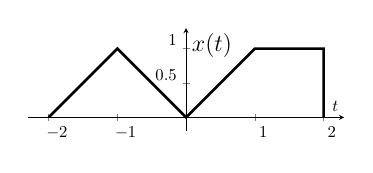
\begin{tikzpicture}[scale=0.6,transform shape]
    \begin{axis}[
        x=0.12\textwidth,y=0.12\textwidth,
    	axis y line=center,
    	axis x line=middle,
    	xlabel=$t$,ylabel={\Large $x(t)$},
    	xmin=-2.3,xmax=2.3,
    	ymin=-.2,ymax=1.3,
    	xticklabel style = {xshift=5},
    	yticklabel style = {yshift=5},
    	]
    	\addplot[
    	black,
    	ultra thick
    	] coordinates {
    	    (-2,0) (-1,1) (0,0) (1,1) 
    	    (2,1) (2,0)
    	} ;
    \end{axis}
\end{tikzpicture}}
    \end{align*}
\end{ejercicio}

\begin{ejercicio}
    Para cada una de las siguientes señales determinar el valor de la variable independiente para el cual la parte par de la señal es cero.
    \begin{align*}
        \inciso & u(n) - u(n-4) & 
        \inciso & \sin\left(\frac{1}{2}t\right) &
        \inciso & \left(\frac{1}{2}\right)^n u(n-3) &
        \inciso & e^{-5t}u(t+2)
    \end{align*}
\end{ejercicio}

\begin{ejercicio}
    Demostrar las siguientes propiedades sobre la paridad las señales en el tiempo continuo:
    
    \inciso Si $x(t)$ es impar, entonces su valor medio es cero:
    \begin{equation*}
        \int_{-\infty}^{\infty} x(t) \, dt = 0
    \end{equation*}
    
    \inciso Si $x(t)$ es par, entonces:
    \begin{equation*}
        \int_{-\infty}^{\infty} x(t) \, dt = 2 \int_{0}^{\infty} x(t) \, dt = 2 \int_{-\infty}^{0} x(t) \, dt
    \end{equation*}

    \inciso Si $x_1(t)$ es par y $x_2(t)$ es impar, entonces $x_1(t)x_2(t)$ es impar.

    \inciso Si $x_1(t)$ es par y $x_2(t)$ es par, entonces $x_1(t)x_2(t)$ es par.

    \inciso Si $x_1(t)$ es impar y $x_2(t)$ es impar, entonces $x_1(t)x_2(t)$ es par.

\vspace*{1em}

\noindent Estos resultados también se extienden para las señales en el tiempo discreto.
\end{ejercicio}


\begin{ejercicio}
    Determinar la energía total, la potencia total, la potencia media y el valor medio de las siguientes señales:
    \begin{align*}
        \inciso & e^{j\frac{2\pi}{8} t} + 2 & 
        \inciso & \sin(\pi t) + \sin\left(\frac{2\pi}{3} t\right) &
        \inciso & e^{-\frac{t^2}{2}} \\
        \inciso & 2^{-n}u(n) &
        \inciso & \cos\left(\frac{2\pi}{8} n\right)
    \end{align*}
\end{ejercicio}

\begin{ejercicio}
    Graficar en \Keyboardsym las siguientes señales de tiempo discreto y determinar si son periódicas o no:
    \begin{align*}
        \inciso & \cos\left(\frac{2\pi}{12} n\right) & \inciso & 2^n u(n) \\
        \inciso & 2^{-n} u(-n+2) & \inciso & \cos\left(\frac{\pi}{3} n \right) u(n-2) \\ 
        \inciso & \cos\left(\frac{1}{6} n\right) & \inciso & \parbox{.5\textwidth}{$x(n)$ definida como las muestras de una senoidal de frecuencia 10Hz muestreada con $T_s=\frac{1}{1000\mathrm{Hz}}$} \\
        \inciso & x(n) = \sum_{k=0}^{50}\cos\left(\frac{\pi k}{32}n\right) & \inciso & x(n) = \sum_{k=0}^{50} \Realpart{a_ke^{\frac{\pi k}{32}n}}\; \mathrm{con}\; a_k = \frac{1}{\pi k} \sin\left(\frac{\pi}{4} k\right)  \\ 
        \inciso & x(n) = \sum_{k=0}^{50}\cos\left(\frac{\pi f(k)}{2}n\right)\; \mathrm{con} & & \hspace{-2.5em} f(k) = 10 \tan\left(\frac{3\pi}{400} k\right)
    \end{align*}

\end{ejercicio}

\begin{ejercicio}
Evaluar, si es posible, las siguientes sumas y expresar su respuesta en forma cartesiana y polar. Implementar una función en \Keyboardsym que obtenga la suma geométrica para cualquiera de ellas. 

\begin{align*}
\inciso & \sum_{n=-2}^7 e^{j\frac{\pi}{2}n} & 
\inciso & \sum_{n=0}^9 \cos\left(\frac{\pi}{3}n\right) &
\inciso & \sum_{n=0}^9 \left(\frac{1}{2}\right)^n e^{j\frac{\pi}{8}n} & \hfill \\[.5em]
\inciso & \sum_{n=0}^\infty a^n e^{j\frac{\pi}{2}n},\; |a| < 1 & 
\inciso & \sum_{n=-4}^\infty \left(\frac{4}{3}\right)^n e^{j\frac{3\pi}{4}n} &
\end{align*}
\end{ejercicio}

\begin{ejercicio}
Sea la señal discreta $x(n)$
\begin{center}
    \input{01_señales/plots/1-discrete_signal}
\end{center}

Graficar cada una de las siguientes señales. Implementar en \Keyboardsym una función que grafique cada una de ellas a partir de una $x(n)$ genérica.

\begin{align*}
    \inciso & x(n) u(2-n) & 
    \inciso & x(n-1) \delta(n-3) & 
    \inciso & \frac{1}{2}x(n) + \frac{1}{2}(-1)^n x(n) \\
    \inciso & x(3n + 1) &
    \inciso & x(3 - n) &
    \inciso & x\left((n-1)^2\right)
\end{align*}

\end{ejercicio}

\begin{ejercicio}
    Implementar en \Keyboardsym \emph{sin utilizar bucles} una función que, dada una señal $x(n)$ y un $N_0\in \mathbb{Z}$, obtenga $y_1(n)=x(N_0n)$ y 
    \begin{equation*}
    y_2(n) = \begin{cases}
    x(n/N_0) & \mbox{si $n$ es múltiplo de $N_0$ } \\
    0 & \mbox{en otro caso}
    \end{cases}
    \end{equation*}
\end{ejercicio}

\begin{ejercicio}
Sea $x(n)$ una señal de tiempo discreta, y sean $y_1(n) = x(2 n)$ y 
\begin{equation*}
y_2(n) = \begin{cases}
x(n/2) & \mbox{si $n$ es par} \\
0 & \mbox{en otro caso}
\end{cases}
\end{equation*}
Determinar si las siguientes afirmaciones son verdaderas o falsas y justificar con demostración o contraejemplo según corresponda. Obtener el período fundamental de $y_1(n)$ y $y_2(n)$.

\inciso Si $x(n)$ es periódica, entonces $y_1(n)$ es periódica.

\inciso Si $y_1(n)$ es periódica, entonces $x(n)$ es periódica.

\inciso Si $x(n)$ es periódica, entonces $y_2(n)$ es periódica.

\inciso Si $y_2(n)$ es periódica, entonces $x(n)$ es periódica.

\end{ejercicio}

\begin{ejercicio}
Sea $x(t)=e^{j\omega_0t}$ la señal exponencial compleja en tiempo continuo con período fundamental $T_0=\frac{2\pi}{\omega_0}$. Considere la señal discreta obtenida al tomar muestras de $x(t)$ equiespaciadas:
\begin{equation*}
    x_d(n) = x(nT_s) = e^{j\omega_0t}\big|_{t=nT_s} = e^{j\omega_0nT_s}
\end{equation*}

\inciso Demostrar que $x_d(n)$ es periódica si y sólo si $\frac{T_0}{T_s}$ es un número racional.

\inciso Determinar el período y la frecuencia fundamental de $x_d(n)$ cuando ésta es periódica. Expresar la frecuencia fundamental como una fracción de $T_0$.

\inciso ¿Cuántos periodos de $T_0$ se necesitan para obtener las muestras que forman un solo período de $x_d(n)$ en el caso en que ésta última es periódica?
\end{ejercicio}

\begin{ejercicio}
    Indicar si las siguientes afirmaciones son verdaderas o falsas:
    
    \inciso La suma de dos señales senoidales de tiempo continuo de frecuencias $f_1$ y $f_2$ es siempre una señal periódica. 
    
    \inciso La suma de dos señales senoidales de tiempo discreto de frecuencias $f_1$ y $f_2$ es siempre una señal periódica. 
    
\end{ejercicio}


